\documentclass{article}
\usepackage[spanish]{babel}

\usepackage[a4paper,bottom=3cm,top=2.5cm,foot=1.5cm,left=1.75cm,right=1.75cm]{geometry}

\usepackage{fontspec}
\setmainfont[Mapping=tex-text]{LinLibertineO}
\newfontfamily\ipa{LinLibertineO}
\setsansfont[Scale=MatchLowercase]{Carlito}
\setmonofont[Scale=MatchLowercase]{DejaVu Sans Mono}

\usepackage{url}
\usepackage{graphicx}
\usepackage{longtable}

\usepackage{color}
\usepackage{colortbl}

\usepackage[table]{xcolor}
\usepackage{booktabs}

\usepackage{lastpage}
\usepackage{datetime}
\usepackage{textpos}
\usepackage{xltxtra}

\definecolor{gris}{rgb}{0.4,0.4,0.4}
\definecolor{morado}{cmyk}{0.09,1,0,0.3}
\definecolor{azul}{cmyk}{1,0.64,0,0.06}


\usepackage{fancyhdr}
\pagestyle{fancy}

% headers y footers
% borramos los estandares
\fancyhf{}
% y le sacamos esa horrible raya que viene por default
\renewcommand{\headrulewidth}{0pt}
\renewcommand{\footrulewidth}{0pt}

% numero de pagina
\fancyfoot[R]{\oldstylenums{\thepage}/\oldstylenums{\pageref{LastPage}}\quad\quad}

\usepackage{hyperref}
\hypersetup{pdftitle={Ramiro Vignolo--Curriculum Vitae}, pdfauthor={Ramiro Vignolo}, pdfkeywords={}, pdfborder={0 0 0}}

% background
\usepackage{eso-pic}
\newcommand\BackgroundPic{
\put(0,0){
\parbox[b][\paperheight]{\paperwidth}{%
\vfill
\centering

\includegraphics{logos/back.pdf}%
\vfill
}}}

% longitudes
\newlength{\chico}
\setlength{\chico}{0.5cm}

\newlength{\grande}
\setlength{\grande}{1.0cm}

\newlength{\ancholeft}
\setlength{\ancholeft}{1.7cm}
\newlength{\anchomain}
\setlength{\anchomain}{13.0cm}
\newlength{\anchoright}
\setlength{\anchoright}{1.5cm}

\newlength{\anchomainright}
\setlength{\anchomainright}{\anchomain}
\addtolength{\anchomainright}{\anchoright}

\newlength{\anchoparrafo}
\setlength{\anchoparrafo}{11.5cm}

\newcommand{\seccionpersonal}[1]{%
\vspace{0.7cm plus 0.2cm minus 0.3cm}
\begin{Large}\textcolor{azul}{\textsc{#1}}\end{Large}
\textcolor{morado}{\hrule}
\vspace{0.2cm plus 0.2cm minus 0.1cm}}

\newcommand{\personalfield}[2]{
\hspace{\chico}\gris{#1}

\smallskip
% \par

\hspace{\grande}{#2}
}



\newenvironment{secciondoscol}[1]{%
% \rowcolors{2}{black!2}{black!0}
\begin{longtable}{p{\ancholeft}p{\anchomainright}}
\multicolumn{2}{l}{
\vspace{0.1cm plus 0.1cm minus 0.1cm}
\hspace{0.25cm}\begin{Large}\textcolor{azul}{\textsc{#1}}\end{Large}
\vspace{-0.1cm}
}
\\
\hline
\vspace{0.2cm plus 0.2cm minus 0.1cm}
\endfirsthead
\multicolumn{2}{l}{
\hspace{0.25cm}\begin{Large}\textcolor{azul}{\textsc{#1}}\end{Large}~~\textcolor{azul}{\textsc{(cont.)}}}\\
\hline 
\vspace{0.2cm plus 0.2cm minus 0.1cm}
\endhead
}{
\end{longtable}
}


\newenvironment{secciontrescol}[1]{%
% \rowcolors{2}{black!2}{black!0}
\begin{longtable}{p{\ancholeft}p{\anchomain}p{\anchoright}}
\multicolumn{3}{l}{
\vspace{0.1cm plus 0.1cm minus 0.1cm}
\hspace{0.25cm}\begin{Large}\textcolor{azul}{\textsc{#1}}\end{Large}
\vspace{-0.1cm}
}
\\
\hline
\vspace{0.2cm plus 0.2cm minus 0.1cm}
\endfirsthead
\multicolumn{3}{l}{
\hspace{0.25cm}\begin{Large}\textcolor{azul}{\textsc{#1}}\end{Large}~~\textcolor{azul}{\textsc{(cont.)}}}\\
\hline 
\vspace{0.2cm plus 0.2cm minus 0.1cm}
\endhead
}{
\end{longtable}
}


\newcommand{\filadosendos}[2]{
 \hfill \textcolor{gris}{\textsf{\small{#1}}} & {\raggedright #2} \\
}
\newcommand{\filadosentres}[2]{
 \hfill \textcolor{gris}{\textsf{\small{#1}}} & \multicolumn{2}{p{\anchomainright}}{\raggedright #2} \\
}
\newcommand{\filatresentres}[4]{
 \hfill \textcolor{gris}{\textsf{\small{#1}}} & {\raggedright #2} & {%
\begin{center}\begin{textblock*}{\linewidth}(0cm,{#4}){#3}\end{textblock*}\end{center}%
} \\
}

\newcommand{\filasep}{ & \\}

% TODO: poner el idioma de babel
\newcommand{\paper}[6]{\filatresentres{#1}{\emph{#3}\\#2\\#4}{\href{#5}{\includegraphics[width=1.2cm]{qr/#6}}}{-0.5cm} \\}
\newcommand{\report}[6]{\filatresentres{#1}{\emph{#3}\\#2\\#4}{\href{#5}{#6}}{-0.5cm} \\}
\newcommand{\congreso}[2]{\filadosentres{#1}{#2}\nopagebreak}
\newcommand{\presentacion}[4]{\filatresentres{}{\emph{#2}\\#1}{\href{#3}{\includegraphics[width=1.2cm]{qr/#4}}}{-0.5cm} \\}
\newcommand{\software}[3]{\filatresentres{#1}{#2}{\href{#3}{\includegraphics[width=1.2cm]{qr/#1}}}{-0.5cm} \\}

\newcommand{\gris}[1]{%
\textcolor{gris}{\textsf{#1}}}

\newcommand{\azul}[1]{%
\textcolor{azul}{\textsf{#1}}}

\newcommand{\titulo}[1]{
\thispagestyle{empty}
\begin{center}
\textcolor{azul}{\Huge{\textbf{#1}}}\\
\vspace{0.1cm plus 0.05cm minus 0.05cm}
\textcolor{gris}{\Large{\textsc{Curriculum Vit\ae}}}
\end{center}
\vspace{0.25cm plus 0.15cm minus 0.1cm}
}

\arrayrulecolor{morado}

% \newcommand{\CC}{C\nolinebreak\hspace{-.05em}\raisebox{.4ex}{\tiny\bf +}\nolinebreak\hspace{-.10em}\raisebox{.4ex}{\tiny\bf +}}
\def\CC{{C\nolinebreak[4]\hspace{-.05em}\raisebox{.4ex}{\tiny\bf ++}}}


\begin{document}
\AddToShipoutPicture{\BackgroundPic}
\titulo{Ramiro Vignolo}

% -=-=-=-=-=-=-=-=-=-=-=-=-=-=-=-=-=-=-=-=-=-=-=-=-=-=-=-=-=-=-=-=-=-=-=-=-=-=-=-=-=-=
\seccionpersonal{Información personal}
% -=-=-=-=-=-=-=-=-=-=-=-=-=-=-=-=-=-=-=-=-=-=-=-=-=-=-=-=-=-=-=-=-=-=-=-=-=-=-=-=-=-=

\vspace{0.5cm plus \chico minus \chico}

\begin{minipage}{0.3\linewidth}
\personalfield{Nombre completo}{Ramiro Vignolo}
\par\vspace{\chico}
\personalfield{Fecha y lugar de nacimiento}{\formatdate{14}{12}{1990}}
\personalfield{}{Córdoba, Argentina}
\par\vspace{\chico}
\personalfield{DNI}{35.573.779}
\par\vspace{\chico}
\personalfield{Estado civil}{Soltero}
\vspace{1cm}
\end{minipage}
\begin{minipage}{0.4\linewidth}

% \hspace{\chico}\gris{Información de contacto}
% \par
\begin{center}
\href{http://www.tecna.com}{
\includegraphics[width=4.5cm]{logos/logo-tecna}}\\

\smallskip

\textsf{Ramiro Vignolo}
\par
\textsf{Ingeniero S/Sr Nuclear}
\end{center}

\smallskip

\hspace{1.25cm}
\begin{minipage}{7cm}
Mariscal José A. Sucre 2600, 4to A\\
Belgrano, Buenos Aires\\
Argentina
\end{minipage}

\begin{center}
+54 9 11 6482 4868\\
\textcolor{azul}{\texttt{ramirovignolo@gmail.com}}\\

+54 11 4347 0300 int. 3455\\
\textcolor{azul}{\texttt{rvignolo@tecna.com}}

\end{center}
\end{minipage}
\begin{minipage}{0.2\linewidth}
\begin{center}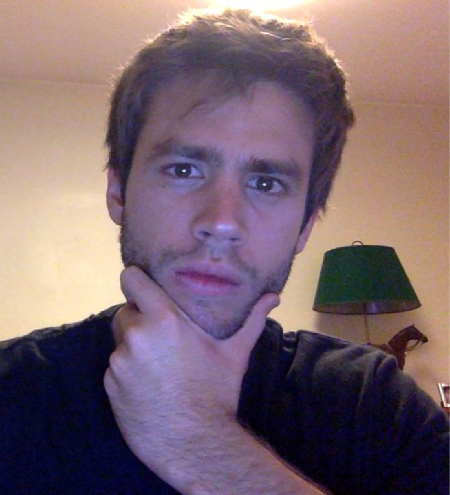
\includegraphics[width=3.5cm]{rvignolopic.png}\end{center}
\end{minipage}

\vspace{1cm plus \grande minus \grande}

% -=-=-=-=-=-=-=-=-=-=-=-=-=-=-=-=-=-=-=-=-=-=-=-=-=-=-=-=-=-=-=-=-=-=-=-=-=-=-=-=-=-=
\begin{secciontrescol}{Formación académica}

\filatresentres{2013}{%
\emph{Ingeniero Nuclear}

Instituto Balseiro, Universidad Nacional de Cuyo, Comisión Nacional de Energía Atómica. San Carlos de Bariloche.\\
Tesis: \href{http://ricabib.cab.cnea.gov.ar/467/}{\emph{Diseño Conceptual del Núcleo de un Reactor de Investigación Compacto.}}\\
Directores: Dr.~Eduardo Villarino e Ing.~Daniel Hergenreder.\\
Departamento de Ingeniería Nuclear de INVAP S.E.\\
Promedio académico: 8.40/10.
}{\href{http://www.ib.edu.ar/index.php/el-balseiro/sobre-el-ib.html}{
\includegraphics[width=0.8cm]{logos/ib}}}{-0.6cm}

\filasep

\filadosentres{2011}{%
Completados los dos primeros años de Ingeniería Aeronáutica.\\
Universidad Tecnológica Nacional, Facultad Regional Haedo.\\
Promedio académico: 9.20/10.
}

\filasep

\filadosentres{2009}{%
\emph{Bachiller Polimodal en Ciencias Naturales}\\
Instituto Social Militar Dr. Dámaso Centeno.
}
\end{secciontrescol}


% -=-=-=-=-=-=-=-=-=-=-=-=-=-=-=-=-=-=-=-=-=-=-=-=-=-=-=-=-=-=-=-=-=-=-=-=-=-=-=-=-=-=
\begin{secciondoscol}{Idiomas}
 \filadosendos{Inglés}{Habla, lee y escribe con fluidez.}
\end{secciondoscol}


% -=-=-=-=-=-=-=-=-=-=-=-=-=-=-=-=-=-=-=-=-=-=-=-=-=-=-=-=-=-=-=-=-=-=-=-=-=-=-=-=-=-=
\begin{secciondoscol}{Premios y becas}

 \filadosendos{2011--2014}{Beca de la Comisión Nacional de Energía Atómica para cursar la carrera de Ingeniería Nuclear en el Instituto Balseiro.\\}

\end{secciondoscol}

% -=-=-=-=-=-=-=-=-=-=-=-=-=-=-=-=-=-=-=-=-=-=-=-=-=-=-=-=-=-=-=-=-=-=-=-=-=-=-=-=-=-=
\begin{secciondoscol}{Lenguajes de programación}
 \filadosendos{C}{Nivel avanzado.}
 \filadosendos{\CC}{Nivel intermedio - avanzado.}
 \filadosendos{Python}{Nivel intermedio.}
 \filadosendos{Fortran}{Nivel intermedio.}
 \filadosendos{\LaTeX}{Nivel avanzado.}
 \filadosendos{Bash}{Nivel intermedio.}
 \filadosendos{AWK}{Nivel intermedio.}
\end{secciondoscol}

% -=-=-=-=-=-=-=-=-=-=-=-=-=-=-=-=-=-=-=-=-=-=-=-=-=-=-=-=-=-=-=-=-=-=-=-=-=-=-=-=-=-=
\begin{secciontrescol}{Experiencia}

\filadosentres{2017--actual}{%
\azul{BESNA}, Buenos Aires\\
\emph{Consultor de Ingeniería}
}

\filasep

\filadosentres{}{%
Proyectos de ingeniería de detalle para centrales nucleares.
Desarrollo de códigos de cálculo termohidráulicos.
Especialista en cálculos y análisis especiales para reactores nucleares de potencia.
}

\filasep

\filadosentres{}{
\begin{tabular}{rp{\anchoparrafo}}
 Proyecto & Simulación Numérica de un Generador de Vapor del Reactor CAREM-25\\
 Cliente  & Comisión Nacional de Energía Atómica (CNEA)\\
 Período  & 2017--actual \\
\end{tabular}}%
\nopagebreak%

\filadosentres{}{Desarrollo del código de cálculo \emph{hhx} (\textbf{h}elical-coiled \textbf{h}eat e\textbf{X}changer) capaz de simular flujo bifásico en cañerías helicoidales y ser acoplado con herramientas de CFD (ANSYS CFX).}

\filasep

\filatresentres{2014--actual}{%
\azul{TECNA} Estudios y Proyectos de Ingeniería S.A., Buenos Aires\\
\emph{Ingeniero S/Sr Nuclear}
}{\href{http://www.tecna.com}{
\includegraphics[width=0.8cm]{logos/tecna-solo}}}{-0.6cm}
\filadosentres{}{%
Proyectos de ingeniería de detalle para centrales nucleares.
Desarrollo de códigos de cálculo neutrónicos, termohidráulicos y de control.
Especialista en cálculos y análisis especiales para reactores nucleares de potencia.
}

\filasep

\filadosentres{}{
\begin{tabular}{rp{\anchoparrafo}}
 Proyecto & Balance de Planta del Reactor CAREM-25\\
 Cliente  & Comisión Nacional de Energía Atómica (CNEA)\\
 Período  & 2017--actual \\
\end{tabular}}%
\nopagebreak%

\filadosentres{}{Consultoría en las implicancias que tienen los diferentes modos de operación del reactor CAREM-25 sobre el Balance de Planta.}

\filasep

\filadosentres{}{
\begin{tabular}{rp{\anchoparrafo}}
 Proyecto & Servicios Especializados de Ingeniería Nuclear para CNAI-II\\
 Cliente  & Nucleoeléctrica Argentina S.A.\\
 Período  & 2014--2016 \\
\end{tabular}}%
\nopagebreak%

\filadosentres{}{Desarrollo e incorporación del método de las características como aproximación para la resolución de la ecuación de transporte de neutrones al código milonga (incluyendo algoritmos de \emph{ray tracing}).}

\filadosentres{}{Consultoría en temas de cálculos neutrónicos de celda para la obtención de secciones eficaces macroscópicas condensadas y homogeneizadas a partir del código de celda DRAGON y con el fin de modelar adecuadamente el efecto Doppler en reactores de agua pesada.}

\filadosentres{}{Coordinación de desarrollos de ingeniería nuclear en temas de neutrónica de celda o núcleo y termohidráulica en reactores tipo PHWR.}

\filadosentres{}{Consultoría en temas de cálculos neutrónicos cinético-espaciales acoplados a códigos de planta y de control.}

\filadosentres{}{Consultoría en desarrollo de códigos computacionales para realizar cálculos transitorios de seguridad acoplados para la actualización del Informe Final de Seguridad de la Central Nuclear Atucha~I.}

\filadosentres{}{Actualizaciones a al Programa Cinético Espacial eXtendido (pcex) y PCE2c.}

\filadosentres{}{Implementación de sistemas de revisión de versiones (Git y Mercurial) a códigos de cálculo y documentación técnica.}

\filadosentres{}{Reimplementación de la suite de código de cálculo acoplado DyPRA como plugin de wasora para aumentar la flexibilidad y trazabilidad de las ejecuciones (dypra2).}

\filadosentres{}{Soporte de ingeniería a las tareas de subida de potencia de la Central Nuclear Atucha~II. Determinación experimental del coeficiente de reactividad por temperatura del combustible a diferentes niveles de potencia durante la etapa de commissioning de la planta mediante el ajuste de parámetros de modelos matemáticos a datos experimentales.}

\filadosentres{}{Extensión del Programa Cinético Espacial (PCE2c): incorporación de rutinas de extracción e inserción de elementos combustibles durante transitorios de cinética neutrónica espacial.
}

\filasep

\filatresentres{2013--2014}{%
\azul{INVAP S.E.} Departamento de Ingeniería Nuclear, San Carlos de Bariloche \\
\emph{Becario de Grado}
}{\href{http://www.invap.com.ar/en/}{
\includegraphics[width=0.8cm]{logos/invap}}}{-0.6cm}

% \nopagebreak
 \filadosentres{}{ 
\begin{tabular}{rp{\anchoparrafo}}
 Proyecto & Proyecto Integrador de la carrera de Ingeniería Nuclear. \\ 
 Período & 2013--2014 \\
 Tareas &

 Realización de la tesis de grado: \href{http://ricabib.cab.cnea.gov.ar/467/}{\emph{Diseño Conceptual del Núcleo de un Reactor de Investigación Compacto.}} \\
\end{tabular}
}

\filasep
 
\filatresentres{2011--2014}{%
\azul{CNEA} Comisión Nacional de Energía Atómica, Centro Atómico Bariloche \\
\emph{Becario de Grado -- Estudiante}
}{\href{http://www.cnea.gov.ar}{
\includegraphics[width=0.8cm]{logos/cnea}}}{-0.6cm}

\filadosentres{}{Estudios realizados en el Instituto Balseiro bajo la beca otorgada por la Comisión Nacional de Energía Atómica para obtener el título de Ingeniero Nuclear.}

\end{secciontrescol}


% -=-=-=-=-=-=-=-=-=-=-=-=-=-=-=-=-=-=-=-=-=-=-=-=-=-=-=-=-=-=-=-=-=-=-=-=-=-=-=-=-=-=
\begin{secciontrescol}{Publicaciones con referato}

\paper{2016}{Vignolo, R.}{Resolución de la ecuación de transporte mediante el método de las características en el código neutrónico milonga}{III Reunión Anual del Grupo Argentino de Cálculo y Análisis de Reactores\\XLIII Reunión Anual de la Asociación Argentina de Tecnología Nuclear}{https://bitbucket.org/rvignolo/aatn-2016-moc-milonga}{aatn-2016-3}

\paper{2016}{Vignolo, R., Schivo, M.}{Coeficiente Doppler: Comparaciones entre mediciones en la Central Nuclear Atucha~II y cálculos de cinética}{XLIII Reunión Anual de la Asociación Argentina de Tecnología Nuclear}{https://bitbucket.org/rvignolo/aatn-2016-appl-multi-xs}{aatn-2016-2}

\paper{2016}{Vignolo, R., Giuntoli, G., Khatchikian, F.}{Desarrollo de tablas de secciones eficaces dependientes de múltiples parámetros en DRAGON V5 para la Cental Nuclear Atucha~II}{XLIII Reunión Anual de la Asociación Argentina de Tecnología Nuclear}{https://bitbucket.org/rvignolo/aatn-2016-xs-multitabla}{aatn-2016-1}

\paper{2015}{Vignolo, R., San Sebastián, G.}{Implementación de rutinas para la extracción e inserción de elementos combustibles dentro de la plataforma de cálculo DyPRA}{XLII Reunión Anual de la Asociación Argentina de Tecnología Nuclear}{https://bitbucket.org/rvignolo/aatn-2015-ext-ins-eecc}{aatn-2015}

\paper{2014}{Vignolo, R., Villarino, E.}{Conceptual Design of a Compact Nuclear Reactor Core}{XVI meeting of the International Group On Research Reactors}{http://www.igorr.com/scripts/home/publigen/content/templates/Show.asp?P=1000&L=EN}{igorr-2014}

\paper{2014}{Vignolo, R., Villarino, E.}{Diseño Conceptual del Núcleo de un Reactor de Investigación Compacto}{Tesis de grado de la carrera de Ingeniería Nuclear del Instituto Balseiro}{http://ricabib.cab.cnea.gov.ar/467/}{tesis-ib}

\end{secciontrescol}


% -=-=-=-=-=-=-=-=-=-=-=-=-=-=-=-=-=-=-=-=-=-=-=-=-=-=-=-=-=-=-=-=-=-=-=-=-=-=-=-=-=-=
\begin{secciontrescol}{Informes técnicos}
\report{2016}{R. Vignolo, G. Giuntoli, TECNA~S.A.}{Coeficiente Doppler: Comparaciones entre WIMS, DRAGON y la Central Nuclear Atucha~II}{ 10527-N-IT16-318 }{}{}

\report{2016}{R. Vignolo, G. Giuntoli, TECNA~S.A.}{Celda combustible de Atucha~II en DRAGON: Generación de tablas de secciones eficaces}{ 10527-N-IT16-317 }{}{}

\report{2015}{J.P. Gómez Omil, A. Tarazaga, R. Vignolo, G. Theler , TECNA~S.A.}{Cálculo de coeficientes para las ecuaciones puntuales de iodo-135 y xenón-135 a partir de distribuciones espaciales de secciones eficaces y propiedades nucleares}{ 10527-N-IT15-309 }{}{}

\report{2015}{R. Vignolo, J. P. Gómez Omil, A. Tarazaga, TECNA~S.A.}{Cálculo de coeficientes de reactividad y curvas de reactividad de bancos de barras de la Central Nuclear Atucha~I}{ 10527-N-IT15-308 }{}{}

\report{2015}{R. Vignolo, J. P. Gómez Omil, TECNA~S.A.}{Determinación y análisis de la reactividad insertada por el boro proveniente del segundo sistema de extinción de la Central Nuclear Atucha~I para dos y tres lanzas}{ 10527-N-IT15-307 }{}{}

\report{2015}{A. Tarazaga, G. Theler, R. Vignolo, TECNA~S.A.}{Modelado en PCEx de la nube de boro correspondiente al Segundo Sistema de Extinción de la Central Nuclear Atucha~I}{ 10527-N-IT15-306 }{}{}

\report{2015}{R. Vignolo, G. Theler, TECNA~S.A.}{Estimaci\'on del coeficiente de reactividad por temperatura del combustible con n\'ucleo  en equilibrio al 100 por ciento de potencia}{ 10527-N-IT15-109 }{}{}

\report{2014}{R. Vignolo, G. Theler, TECNA~S.A.}{Estimaci\'on del coeficiente de reactividad por temperatura del combustible con n\'ucleo  en equilibrio al 90 por ciento de potencia}{ 10527-N-IT15-108 }{}{}

\report{2014}{R. Vignolo, TECNA~S.A.}{Implementación de rutinas para la extracción e inserción de elementos combustibles en PCE2c dentro de la plataforma DyPRA}{ 10527-N-IT15-202 }{}{}


\end{secciontrescol}

% -=-=-=-=-=-=-=-=-=-=-=-=-=-=-=-=-=-=-=-=-=-=-=-=-=-=-=-=-=-=-=-=-=-=-=-=-=-=-=-=-=-=
\begin{secciontrescol}{Presentaciones en congresos}

\congreso{2016}{III Reunión Anual del Grupo Argentino de Cálculo y Análisis de Reactores, Buenos Aires}%
%
\presentacion{Vignolo, R.}{Taller DRAGON: Aprendiendo a Utilizar DRAGON V5 como código de producción de secciones eficaces}{https://bitbucket.org/rvignolo/taller-dragon-garcar-2016}{garcar-2016-2}

\presentacion{Vignolo, R.}{Resolución de la ecuación de transporte mediante el método de las características en el código neutrónico milonga}{https://bitbucket.org/rvignolo/aatn-2016-moc-milonga-presentacion}{garcar-2016-1}

\congreso{2016}{XLIII Reunión Anual de la Asociación Argentina de Tecnología Nuclear, Buenos Aires}%
%
\presentacion{Vignolo, R., Giuntoli, G., Khatchikian, F.}{Desarrollo de tablas de secciones eficaces dependientes de múltiples parámetros en DRAGON V5 para la Cental Nuclear Atucha~II}{https://bitbucket.org/rvignolo/aatn-2016-xs-multitabla-presentacion}{aatn-2016-1-pres}
%
\presentacion{Vignolo, R., Schivo, M.}{Coeficiente Doppler: Comparaciones entre mediciones en la Central Nuclear Atucha~II y cálculos de cinética}{https://bitbucket.org/rvignolo/aatn-2016-appl-multi-xs-presentacion}{aatn-2016-2-pres}
%
\presentacion{Vignolo, R.}{Resolución de la ecuación de transporte mediante el método de las características en el código neutrónico milonga}{https://bitbucket.org/rvignolo/aatn-2016-moc-milonga-presentacion}{aatn-2016-3-pres}

\congreso{2015}{XLII Reunión Anual de la Asociación Argentina de Tecnología Nuclear, Buenos Aires}%
%
\presentacion{Vignolo, R., San Sebastián, G.}{Implementación de rutinas para la extracción e inserción de elementos combustibles dentro de la plataforma de cálculo DyPRA}{https://bitbucket.org/wasora/wasora}{wasora}

\end{secciontrescol}


% -=-=-=-=-=-=-=-=-=-=-=-=-=-=-=-=-=-=-=-=-=-=-=-=-=-=-=-=-=-=-=-=-=-=-=-=-=-=-=-=-=-=
\begin{secciontrescol}{Desarrollo de software libre}

\software{wasora}{Herramienta computacional para el modelado, análisis y optimización de sistemas dinámicos complejos mediante la definición del problema matemático como expresiones de alto nivel en un archivo de texto}{https://bitbucket.org/wasora/wasora}

\software{milonga}{Transporte y difusión de neutrones con volúmenes y elementos finitos en mallas no estructuradas con especial énfasis en la definición de secciones eficaces macroscópicas como funciones de~$x$, $y$ y~$z$ a través de distribuciones espaciales arbitrarias}{https://bitbucket.org/rvignolo/milonga}

\end{secciontrescol}


% -=-=-=-=-=-=-=-=-=-=-=-=-=-=-=-=-=-=-=-=-=-=-=-=-=-=-=-=-=-=-=-=-=-=-=-=-=-=-=-=-=-=
\begin{secciondoscol}{Asesoramiento}
 \filadosendos{2016}{Vocal Prensa y Comunicación de la Asociación Argentina de Jóvenes Nucleares.\\}
\end{secciondoscol}

% \pagebreak


\vspace{\fill}
\hspace{0.6\linewidth}
\begin{minipage}{0.35\linewidth}
 \begin{center}
 Ramiro Vignolo\\
% version tracking
\immediate\write18{./date.sh > date.tex }
\immediate\write18{./hash.sh > hash.tex }

\makeatletter
\ifcase\pdf@shellescape
  \today\or
  \input{date}\or
  \today\fi

\scriptsize{\texttt{
\ifcase\pdf@shellescape
  unknown revision hash, re-compile with '--shell-escape'\or
  \input{hash}\or
  unknown revision hash, re-compile with '--shell-escape'\fi
}}
\makeatother
 
 \end{center}
\end{minipage}


\end{document}
